\section{Deep Q Networks (DQN)}
\label{sec:DQN}
The first deep reinforcement learning network there has been created in this project is the Deep Q Network. The Deep Q Network was first time described in the paper "playing Atari with Deep reinforcement learning" \cite{DBLP:journals/corr/MnihKSGAWR13} published by DeepMind. In this paper they learned the computer to play Atari 2600 video games. The computer only observed the screen pixels from the game, and received a reward when the game score increased. The result was remarkable, because the games and the goals in the games are very different. The same architecture was used for seven different games. In 3 of the seven games the computer performed better than the best human. 

To understand the problem the Deep Q Network solved, it is easier to use an example, here we use the game Breakout as an example. In this game you control a paddle at the bottom of the screen, and have to clear the bricks in the top of the screen. This is done by bouncing a ball between the paddle and the bricks. Each time a brick is hit it disappears and the game score increases. The game can be seen on figure \Cref{fig:Atari_breakout}

\begin{figure}[H]
	\centering
	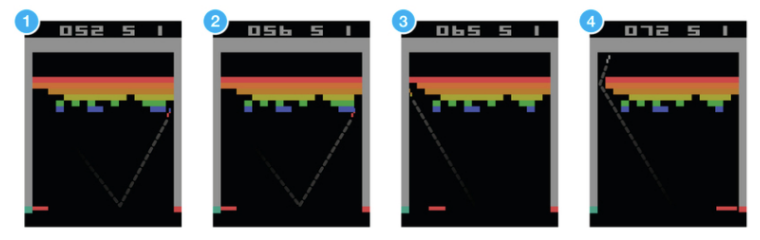
\includegraphics[width=1\textwidth]{Figures/Architecture/DQN/Atari_breakout.png}
	\caption{Atari Breakout game. Image credit: DeepMind\cite{DBLP:journals/corr/MnihKSGAWR13} }
	\label{fig:Atari_breakout}
\end{figure}

To teach a Network how to play this game, the input to the network is the screen images, and the output is the actions of the game: left, right or fire (to launch the ball). One approach to this problem is to treat it as a classification problem - for each screen decide if the paddle should move left, right or press fire. To do this lots of training examples is needed. The problem about this approach is thats really how human learns, we don't need someone to tell us million times which move to choose at each screen. Instead human just need occasional feedback that we did the right thing, and then learn from it ourself. This is the task reinforcement learning tries to solve, more of the reinforcement learning theory can be read in \textbf{Reference to Theory chapter}.

While the idea is quite intuitive, in practice there are numerous challenges. One of the challenges is when hitting a brick and the reward is received, it often has nothing to do with the actions (paddle movement) just before the reward was received. All the work was done when the paddle was positioned correctly and bounced the ball back. This is called the credit assignment problem – i.e., which of the preceding actions was responsible for getting the reward and to what extent.

Another challenge is when a strategy is found and a certain reward is received, should the program stick with that strategy or experiment with something that could lead to a bigger reward. This is called the explore-exploit dilemma – should you exploit the known working strategy or explore other, possibly better strategies. 

The screen pixels obtain most of the relevant information of the game situation, except speed and direction of the ball. This could be covered by having two consecutive screens. 

\subsection{Preprocessing}
The DeepMind paper use preprocessing where the take the last four screen images, resize them to 84x84 and convert to grayscale with 256 gray levels. This will give $256^{84x84x4} \approx 10^{67970}$ possible game states. This will give $10^{67970}$ rows in the imaginary Q-table - more than the number of atoms in the universe. Many pixel combinations never occur, so possible represent it as a sparse table containing only visited states. Most of the states are rarely visited and it would take a lifetime of the universe to the q-table to converge. It should also be possible to have a good guess for Q-values for states we have never seen. 

To do this deep learning comes in to the picture. Neural networks are extremely good at coming up with good features for highly structured data. A way neural networks can be used in reinforcement learning is it could represent the Q-function, where it takes the state (four game screens) and action as an input and output the corresponding Q-value. Another way is to only take game screens as input, and output the Q-value for each possible action. The second approach has the advantages, that if we want to perform a Q-value update or choose the action with the highest Q-value, it can be done by only doing one forward pass in the network and have all Q-values for all possible actions. The two different approaches to use neural network to represent the Q-function can be seen on \Cref{fig:DQN_two_approach}.              


\begin{figure}[H]
	\centering
	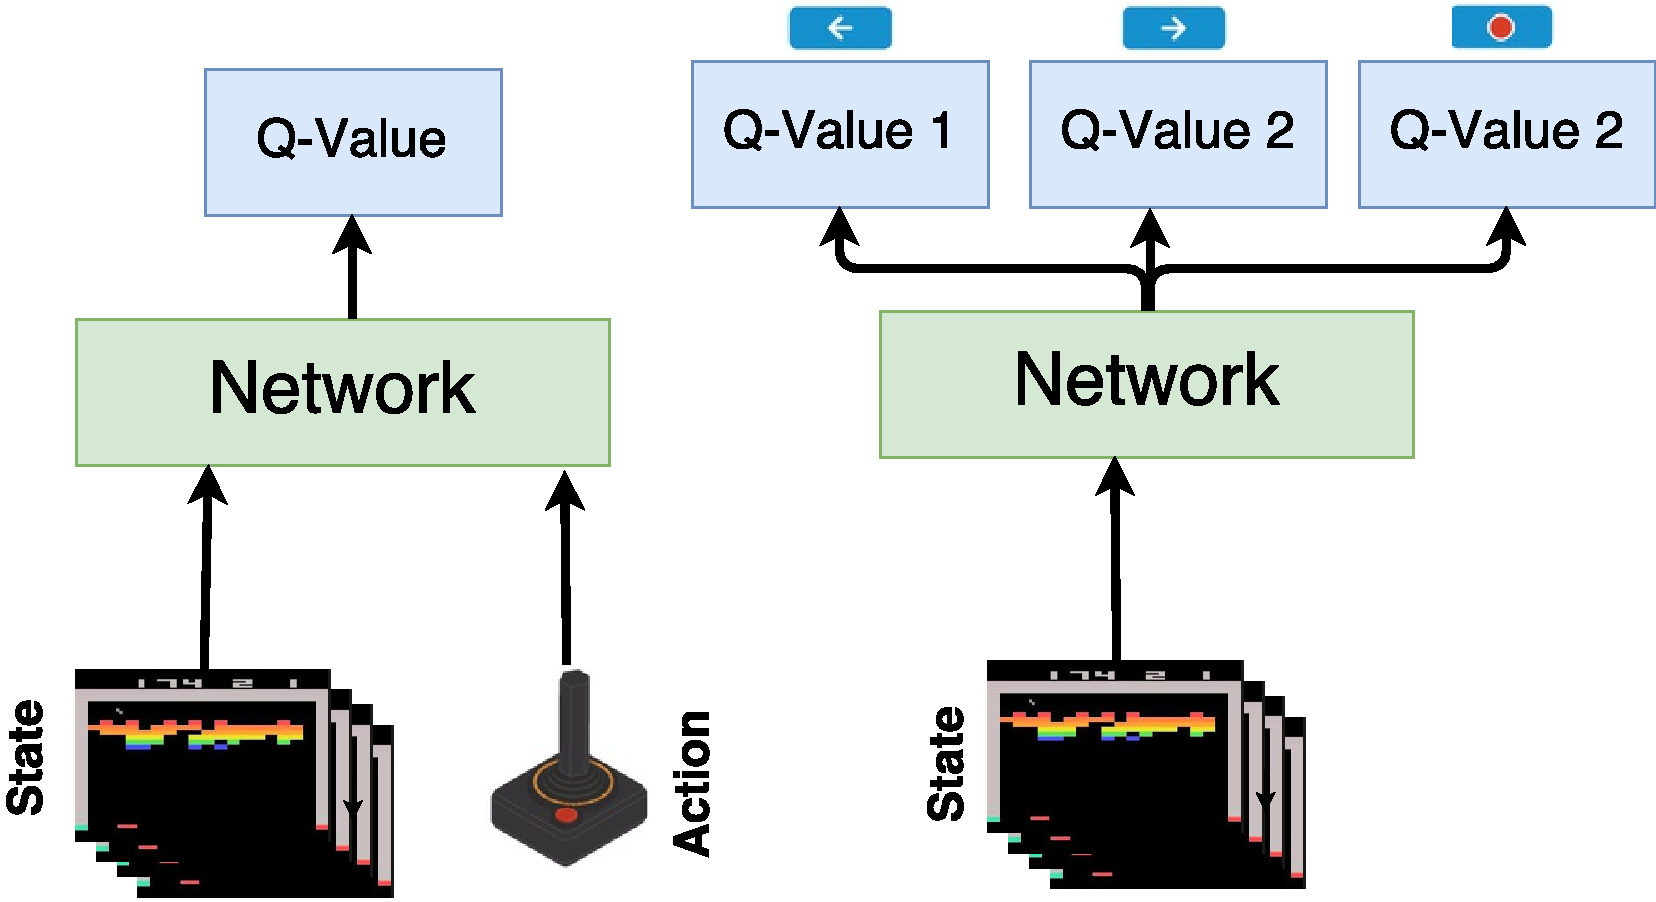
\includegraphics[width=1\textwidth]{Figures/Architecture/DQN/DQN_two_approach.pdf}
	\caption{Left: Naive formulation of deep Q-network. Right: More optimized architecture of deep Q-network, used in DeepMind paper.} 
	\label{fig:DQN_two_approach}
\end{figure}    

\subsection{Network}
The network architecture that DeepMind used can be seen on the table below \Cref{tab:DQN_network}. 

\begin{table}[H]
	\centering
	\caption{Architecture of the Deep Q Network used by DeepMind}
	\label{tab:DQN_network}
	\begin{tabular}{|l|c|c|c|c|c|c|}
		\hline
		\rowcolor[HTML]{9B9B9B} 
		\multicolumn{1}{|c|}{\cellcolor[HTML]{9B9B9B}\textbf{Layer}} & \textbf{Input} & \textbf{Filter size} & \textbf{Stride} & \textbf{Num filters} & \textbf{Activation} & \textbf{Output} \\ \hline
		\cellcolor[HTML]{FFFFFF}\textbf{conv1}                       & 84x84x4        & 8x8                  & 4               & 32                   & ReLU                & 20x20x32        \\ \hline
		\rowcolor[HTML]{C0C0C0} 
		\textbf{conv2}                                               & 20x20x32       & 4x4                  & 2               & 64                   & ReLU                & 9x9x64          \\ \hline
		\cellcolor[HTML]{FFFFFF}\textbf{conv3}                       & 9x9x64         & 3x3                  & 1               & 64                   & ReLU                & 7x7x64          \\ \hline
		\rowcolor[HTML]{C0C0C0} 
		\textbf{fc4}                                                 & 7x7x64         &                      &                 & 512                  & ReLU                & 512             \\ \hline
		\cellcolor[HTML]{FFFFFF}\textbf{fc5}                         & 512            &                      &                 & 18                   & Linear              & 18              \\ \hline
	\end{tabular}
\end{table}

The network can be seen as a classical convolutional neural network with three convolutional layers, followed by two fully connected layers. One of the things which makes this neural network different from the classical neural networks used for image recognition, is no poling layers are used. No pooling layers are used because they buy translation invariance -  the network becomes insensitive to the location of an object in the image. This is okay for image recognition, but for games where the location of the ball is important for deciding the potential reward.  

As seen on \Cref{fig:DQN_two_approach} the input to the network is four 84x84 grayscale game screens. The output of the network are a Q-value for each action, 18 actions for atari games (in breakout there are only 3 actions). The Q-value can be any real number, which make it a regression task. The optimization of the Q-values can be done by a squared error loss. 

\begin{equation}
L=\frac{1}{2}[r+max_{a'}Q(s',a')-Q(s,a)]^2
\end{equation}  

In the squared error loss function is $r+max_{a'}Q(s',a')$ the target, and $Q(s,a)$ is the prediction. Given a transaction <s,a,r,s'>, the Q-table is updated by the following steps:
\begin{enumerate}
	\item Do a feedforward pass for the current state s to get predicted Q-values for all actions.
	\item Do a feedforward pass for the next state s’ and calculate maximum overall network outputs $max_{a'}Q(s',a')$
	\item Set Q-value target for action to $r+max_{a'}Q(s',a')$ (use the max calculated in step 2).For all other actions, set the Q-value target to the same as originally returned from step 1, making the error 0 for those outputs. 
	\item Update the weights using backpropagation.
\end{enumerate}

\subsubsection{Experience Replay}
The approximation of the Q-values using non-linear functions is not very stable. There is many tricks to make i converge. And the problem with this method is it takes long time to converge almost a week on a single GPU. 

The most important tricks is experience replay. During gameplay all the experiences <s, a, r, s’> are stored in a replay memory. While training the network random minibatches are used instead of the recent transition. This breacks the similarity of training samples, and there by avoid the network to reach a local minimum. Experience replay makes the training task more similar to usual supervised learning, which simplifies debugging and testing the algorithm. A way this could be done is by collecting experience from human players, and train on those experiences.
  
\subsubsection{Exploration-Exploitation}
In reinforcement learning the Exploration-Exploitation dilemma, is if the agent should explore or exploit. First when the Q-table or Q-network is initialized randomly, then the prediction of the action is equally random, this is called exploration. As a Q-function converges, it returns more consistent Q-values and the amount of exploration decreases. Q-learning use the exploration as part of the algorithm. But this exploration is “greedy”, it settles with the first effective strategy it finds.

A simple way to do this is to use the $\epsilon$-greedy exploration - with probability $\epsilon$ choose a random action, otherwise go with the “greedy” action with the highest Q-value. DeepMind decreases $\epsilon$ over time from 1 to 0.1. This means in the beginning the system makes random actions to explore the state space maximally, and in the end it settles to a fixed exploration rate.  

\subsubsection{Algorithm}
All this theory end up in an algorithm of the Deep Q Network with experience replay, which can be seen below in \Cref{algo:DQN}.. This is the Algorithm from DeepMind \cite{DBLP:journals/corr/MnihKSGAWR13}.

\begin{algorithm}
	\caption{Deep Q-learning with Experience Replay}
	\label{algo:DQN}
	\begin{algorithmic}[]
		\State initialize replay memory \textit{D}
		\State initialize action-value function \textit{Q} with random weights
		\State observe initial state \textit{s} 
		\Repeat
			\State select an action \textit{a}
				\par with probability $\epsilon$ select a random action otherwise select 
				\par $a = \mathrm{argmax}_{a'}Q(s,a')$
		
			\State carry out action \textit{a}
			\State observe reward \textit{r} and new state \textit{s'}
			\State store experience <\textit{s}, \textit{a}, \textit{r}, \textit{s'}> in replay memory \textit{D}
			\newline
			\State sample random transition <\textit{ss}, \textit{aa}, \textit{rr}, \textit{ss'}>      
			\State calculate target for each minibatch transition
				\par if \textit{ss'} is terminal state then \textit{tt} = \textit{rr} otherwise 
				\par $tt = rr + \gamma \mathrm{max}_{a'}Q(ss',aa')$
			\State train the Q network using $(\textit{tt} - Q(\textit{ss}, \textit{aa}))^2$ as loss	
			\newline
			\State \textit{s} = \textit{s'}
		\Until terminated
	\end{algorithmic}
\end{algorithm}

This is some of the tricks DeepMind has used, to get the Deep Q Network to work, but they use other tricks than these. Some of the other tricks they use is target network, error clipping, reward clipping etc. 

The amazing part of the Deep Q Network is that it learns. Because the Q-function is initialized randomly, it initially outputs doesn't make sense at all. The network then uses this outputs (the maximum Q-value of the next state ) as targets for the network, only occasionally folding in a tiny reward. This is what made the Deep Q Network, the state of the art, when it was published. \cite{DQN_theory} \cite{DQN_Flappy} 

        